\mychapter{Procedimento Experimental}
\label{Cap:Procedimento}

Esse capítulo descreve os dispositivos e a metodologia utilizada na execução dos experimentos, o cenário onde esses experimentos formam realizados e, por fim, os experimentos realizados para aferir parâmetros de funcionamento dos módulos XBee PRO S3B 900HP.

\section{Tecnologias Utilizadas}

Além do módulo XBee PRO S3B 900HP (fig \ref{fig:xbeepro}), foram utilizados na execução dos experimentos: módulos XBee \emph{Explorer}, aeronaves \emph{Phantom 3 Standard}, o \emph{software} XCTU utilizado para a realização dos testes e uma fonte de alimentação externa para alimentar o conjunto módulo XBee + XBee \emph{Explorer}.

As especificações técnicas, bem como o modo de funcionamento, dos módulos XBee já foram discutidos no capítulo \ref{Cap:Xbee}. Os demais materiais utilizados serão descritos a seguir.

\begin{figure}[h!] 
\center
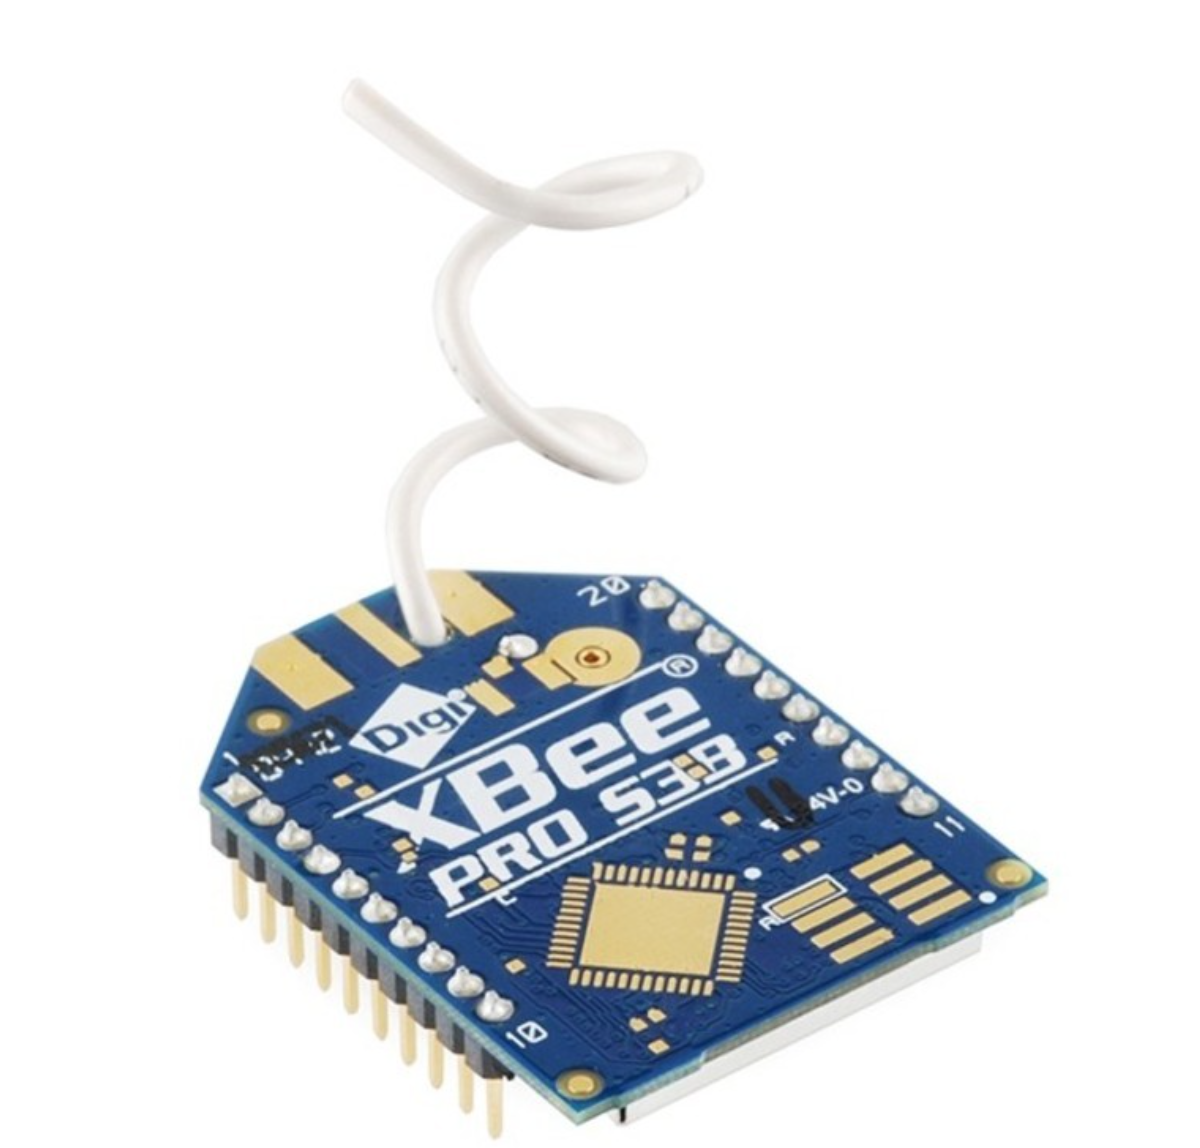
\includegraphics[width=0.7\textwidth]{xbeepro.png}
\caption{Módulo XBee PRO S3B 900HP.} 
\label{fig:xbeepro}
\end{figure}

\subsection{XBee \emph{Explorer}}

O XBee \emph{Explorer} é a \emph{interface} de \emph{hardware} utilizada para conectar um módulo XBee a outros dispositivos, como por exemplo um computador. O módulo adquirido pelo projeto, como mostra a figura \ref{fig:xbeeexplorer}, possui duas formas de acesso ao módulo XBee acoplado a ele, sendo essas uma porta micro usb, utilizada para alimentação e comunicação, ou um conjunto de pinos contendo Rx, Tx, \emph{reset} e os pinos a serem utilizados para alimentação.

Apesar de da voltagem de alimentação dos módulos XBee ser de +3.3 volts, o XBee \emph{Explorer} deve ser alimentado com uma fonte que forneça +5 volts, que é reduzida para a voltagem de alimentação requerida pelo módulo XBee através da circuitaria do \emph{Explorer}.

\begin{figure}[h!] 
\center
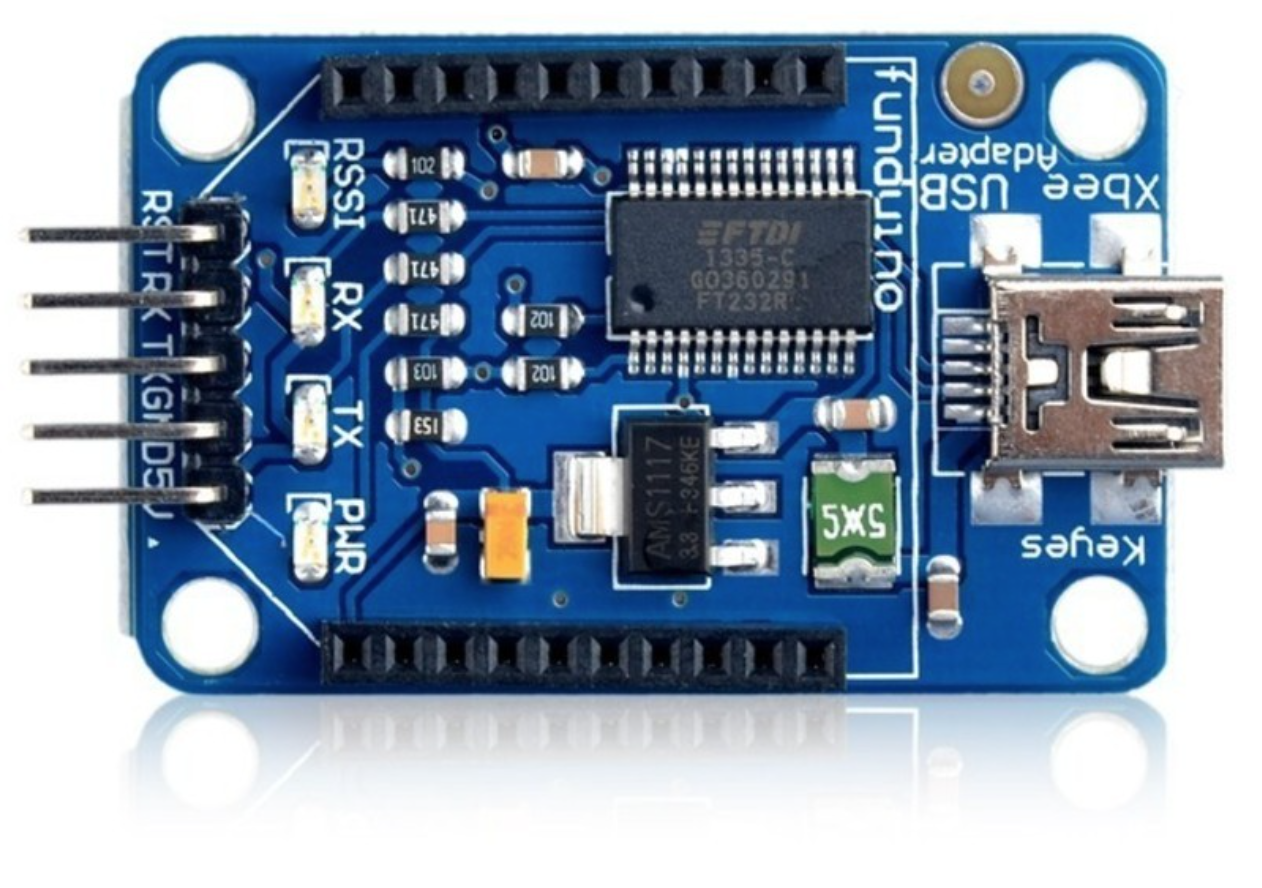
\includegraphics[width=0.7\textwidth]{xbeeexplorer.png}
\caption{XBee \emph{Explorer}.} 
\label{fig:xbeeexplorer}
\end{figure} 

\subsection{Phantom 3 Standard}

Outro dispositivo de grande importância para a realização dos experimentos foram os quadrirrotores do modelo \emph{Phantom 3 Standard} (figura \ref{fig:phantom}) adquiridos pelo projeto e utilizados para variação e medição da distância entre os nós da rede \emph{mesh} formada para a realização dos teste de performance.

As aeronaves são controladas utilizando controle remoto que as acompanha e um \emph{smartphone} rodando o aplicativo DJI Go, que da suporte visual para a operação das aeronaves. Parâmetros como altitude de voo, velocidade vertical e horizontal, nível de bateria, distância entre a aeronave e o operador, entre outros, estão sempre de fácil acesso visual bem como a imagem capturada pela câmera embarcada que é transmitida em tempo real para o operador. 

\begin{figure}[h!] 
\center
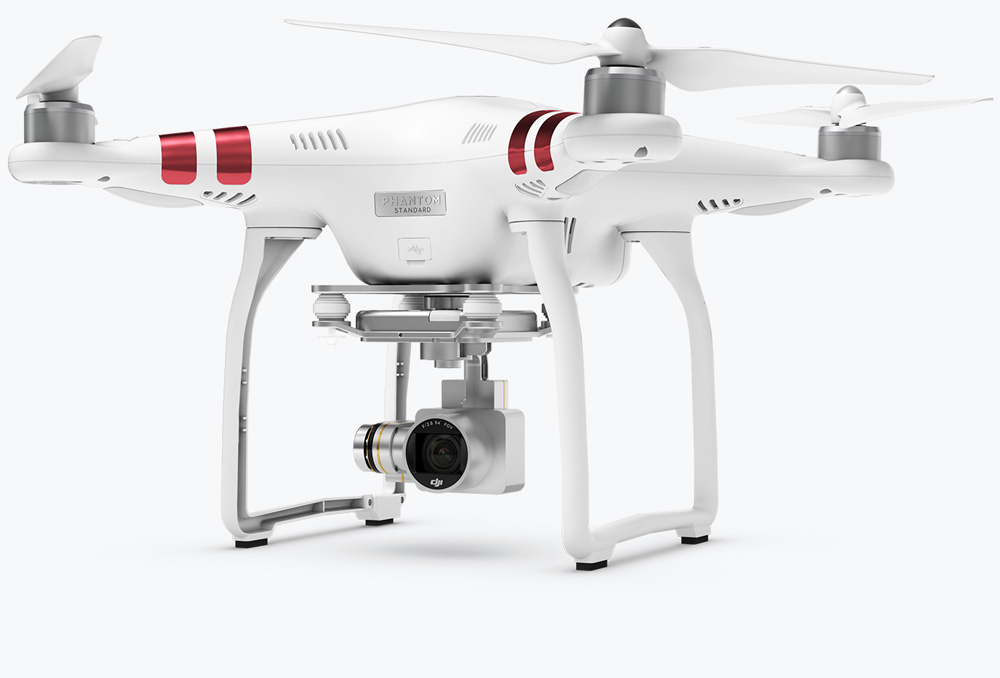
\includegraphics[width=0.7\textwidth]{phatom.jpg}
\caption{Aeronave Phantom 3 \emph{Standard}.} 
\label{fig:phantom}
\end{figure}

\subsection{XCTU}

O XCTU, bevemente apresentado no capítulo \ref{Cap:Xbee}, é o \emph{software}, disponibilizado pela fabricante dos módulos XBee, utilizado para configuração dos dispositivos e que também possui algumas ferramentas para analise da qualidade da rede formada. Ferramentas essas que foram utilizadas nesse trabalho para aferir a qualidade da rede, em especial o teste de força de sinal e o de taxa de transmissão (\emph{throughput}).

As figuras \ref{fig:rangeTest} e \ref{fig:throughput} apresentam, respectivamente, as telas dos testes de força de sinal e taxa de transmissão disponíveis no \emph{software} XCTU.

\begin{figure}[h!] 
\center
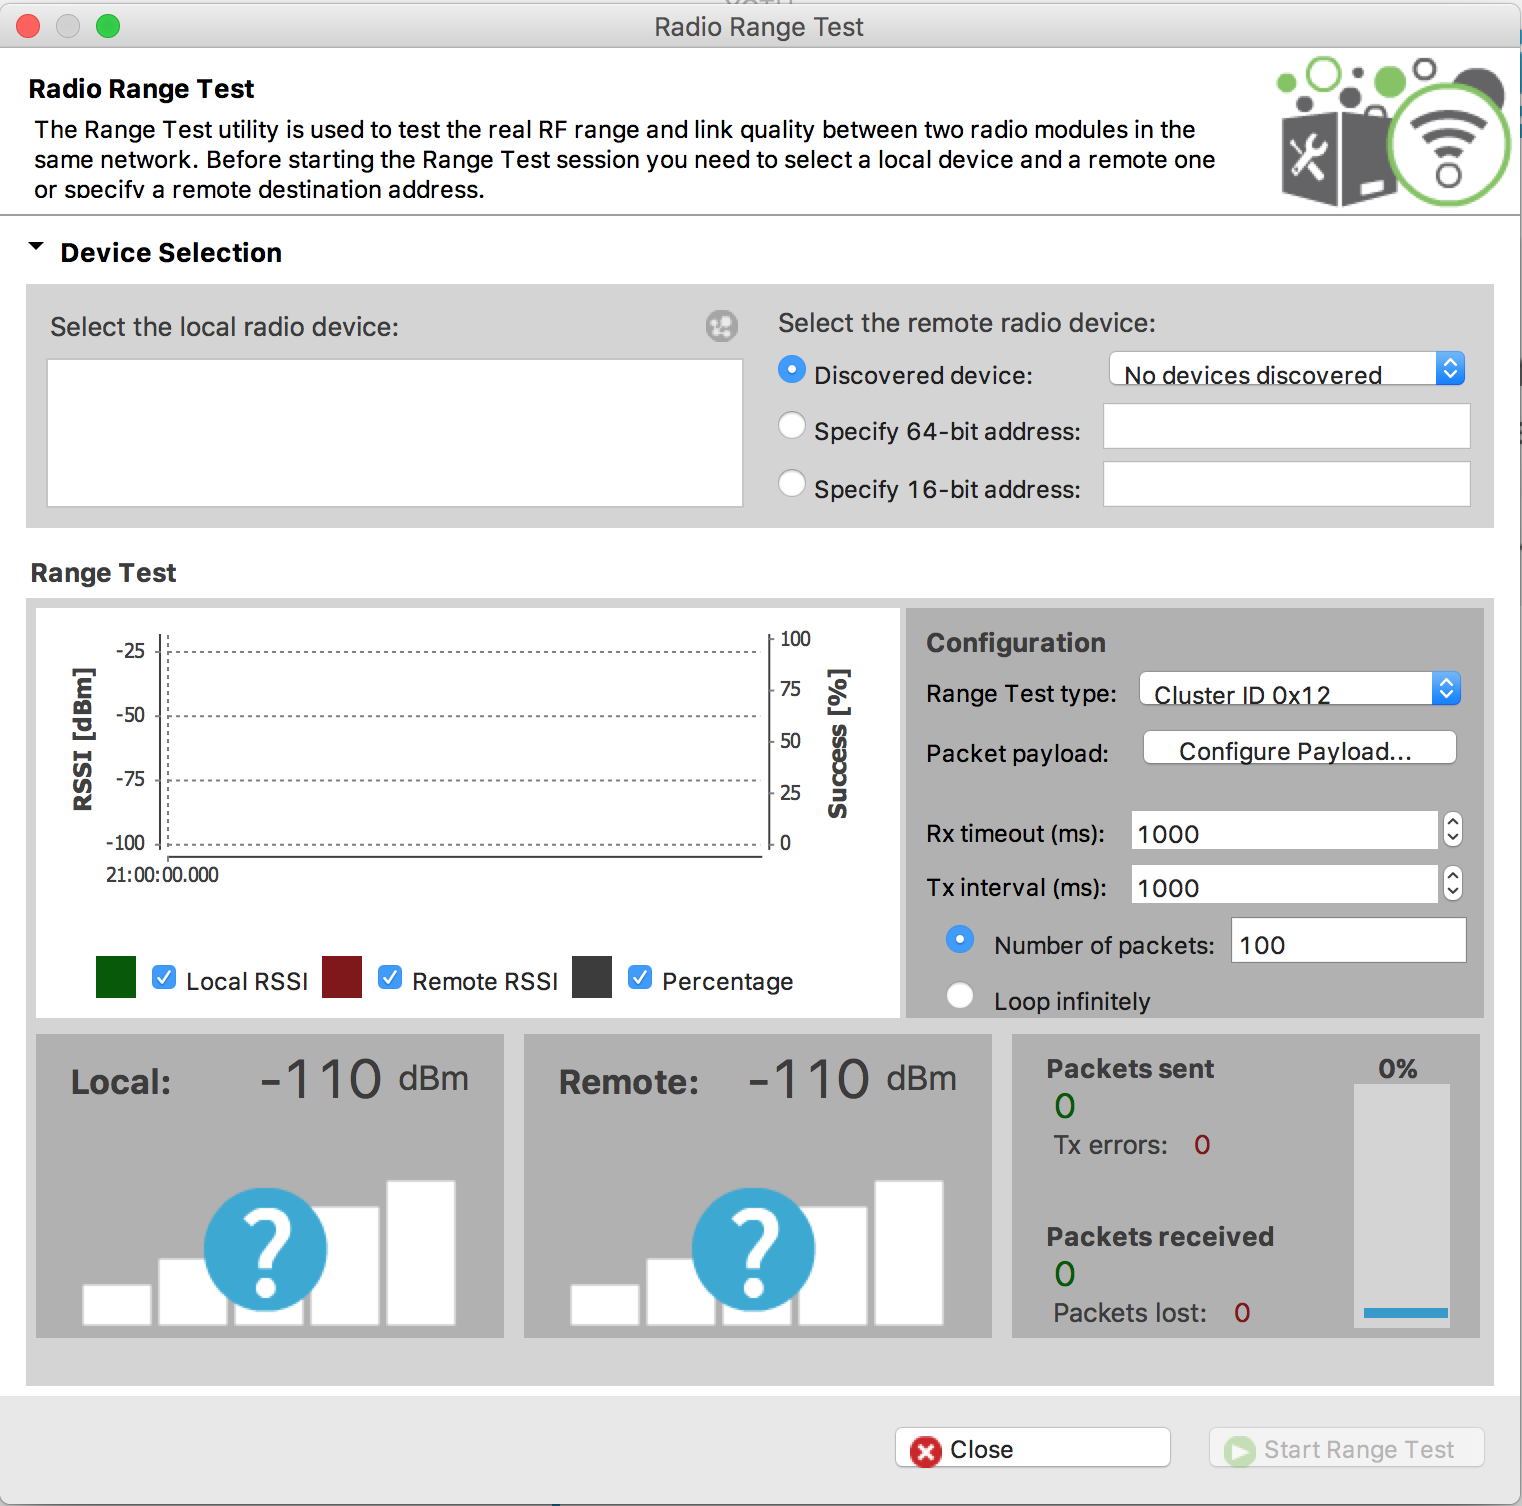
\includegraphics[width=0.7\textwidth]{RangeTest.png}
\caption{Tela do teste de força de sinal.} 
\label{fig:rangeTest}
\end{figure}

\begin{figure}[h!] 
\center
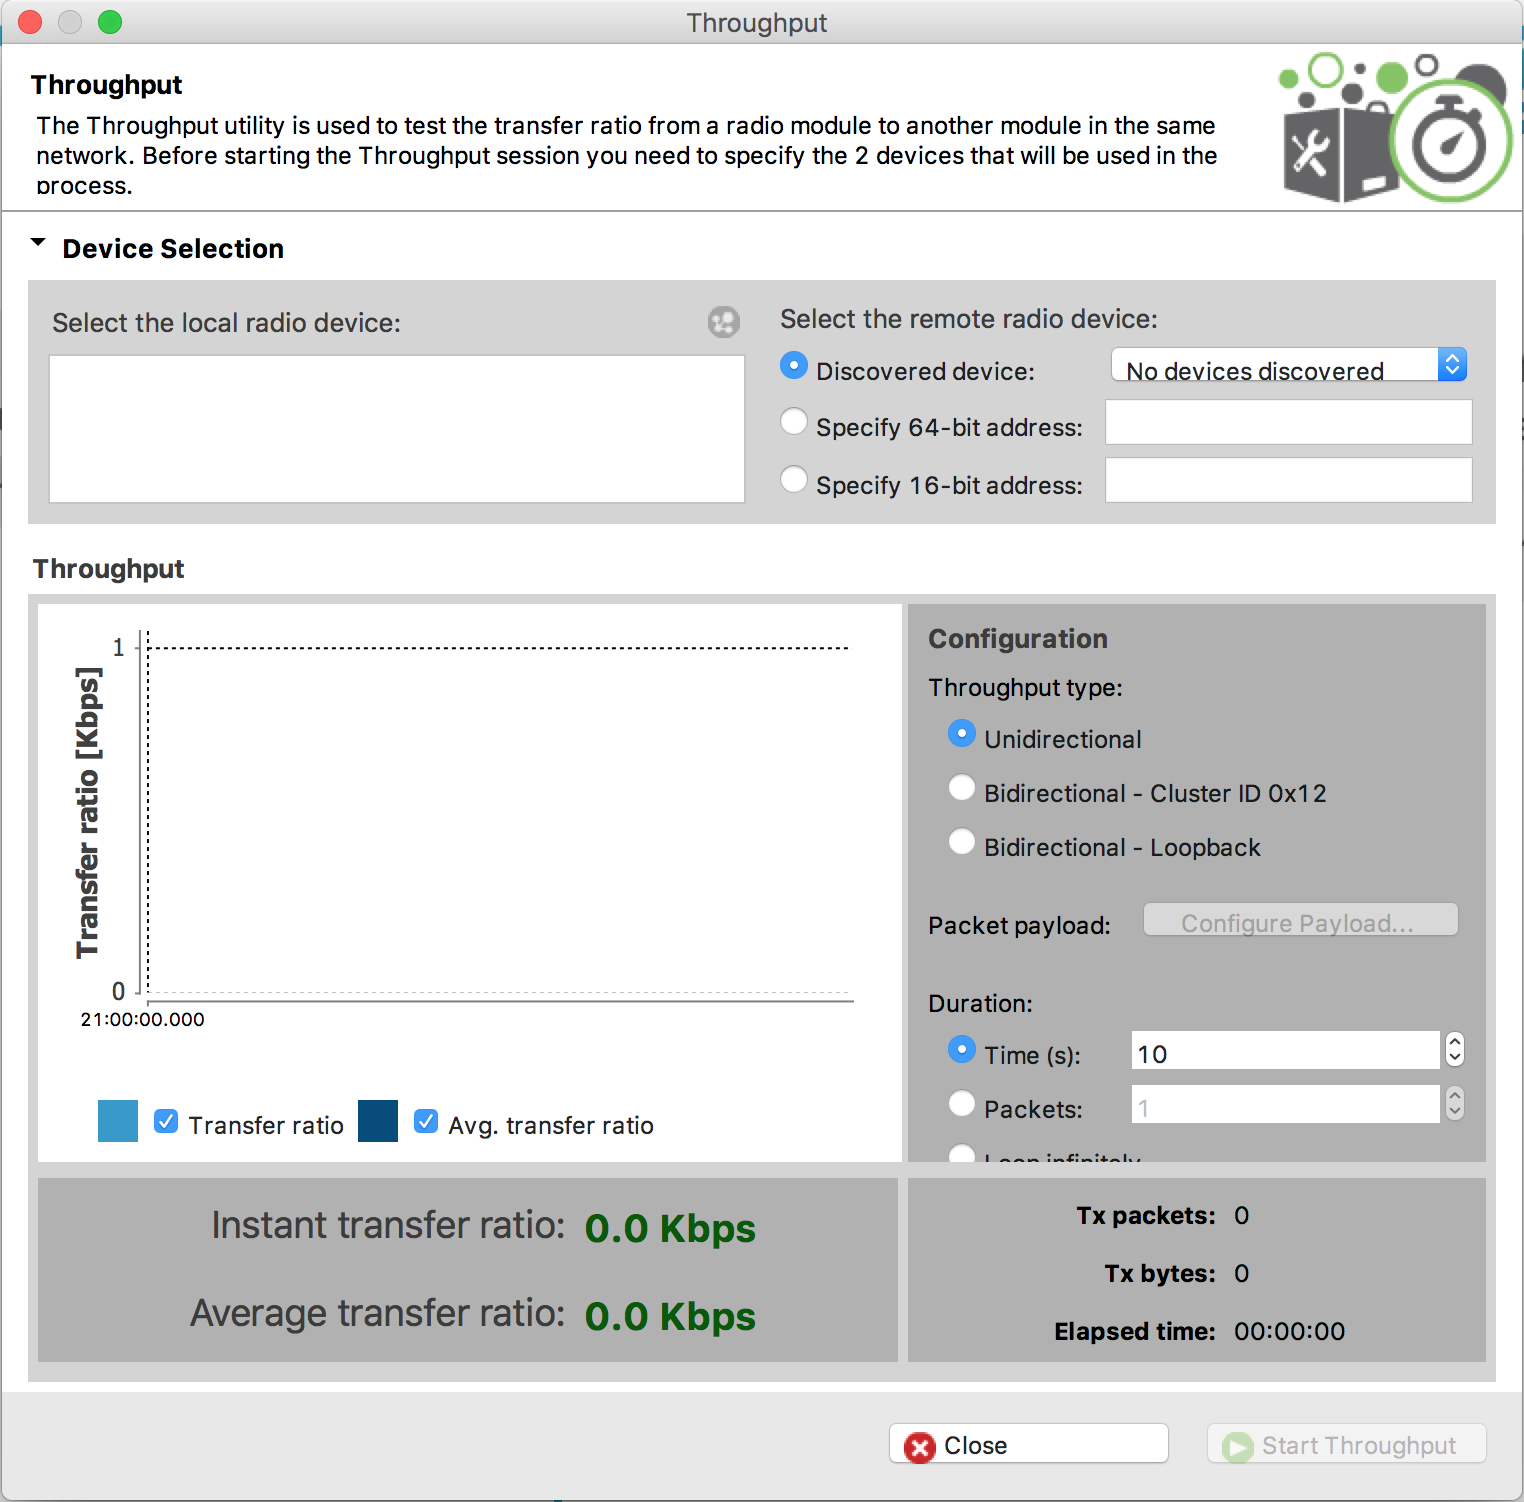
\includegraphics[width=0.7\textwidth]{ThroughputTest.png}
\caption{Tela do teste de taxa de transmissão (\emph{throughput}).} 
\label{fig:throughput}
\end{figure}

\section{Local dos Experimentos}

O local ideal para a realização dos experimentos seria o local onde o sistema final seria utilizado, ou seja, o próprio Centro de Lançamento Barreira do Inferno (CLBI), pois os testes refletiriam as condições especificas de interferência e meio de comunicação onde a rede multi VANTs será operada.

Infelizmente, devido a indisponibilidade de tempo e acesso, os testes de campo aqui apresentados foram realizados em sua maioria no campo central da Universidade Federal do Rio Grande do Norte (UFRN), o que pode ser considerado um ambiente urbano e pode apresentar níveis de interferência de sinal maiores que o ambiente onde a rede será de fato operacionalizada. 

\section{Experimentos Realizados}

No intuito de aferir a qualidade dos \emph{links} e, consequentemente, a rede a qual eles fazem parte, no contexto de um rede multi VANTs, foram realizados múltiplos testes de força de sinal e taxa de transmissão para diferente cenários, sendo eles:

\begin{itemize}
\item Teste de chão
\item Teste em ar a distância fixa
\end{itemize} 

\subsection{Teste de Chão}

Para a realização dos testes de chão, o conjunto de equipamentos necessários (módulo XBee + XBee \emph{Explorer} + bateria portátil) foram afixados ao \emph{Phantom 3 Standard} com o auxílio de fita colante do tipo \emph{silver tape}, como mostra a figura \ref{fig:conjExp}, e um outro módulo XBee foi conectado ao um \emph{notebook} dotado do \emph{software} XCTU, através do XBee \emph{Explorer}.

O aeromodelo, embarcado com os equipamentos requeridos, foi então posicionado em diferentes pontos do campo e os testes de força de sinal e taxa de transferência, disponíveis no XCTU, foram executados e seus resultados armazenados para analise. Os testes foram realizados 5 vezes para cada distância e a média desses cinco resultados foram considerados para análise de desempenho. 
 
\subsection{Teste em Ar a Distância Fixa}

Assim como nos testes de chão, com o auxilio de fita colante, um módulo XBee, um XBee \emph{Explorer} e uma bateria portátil foram afixados ao aeromodelo (fig. \ref{fig:conjExp}) e um outro módulo XBee foi conectado, através do XBee \emph{Explorer}, a um \emph{notebook} dotado do \emph{software} XCTU. 

Uma vez que todos os equipamentos estavam devidamente conectados, a aeronave \emph{Phantom} foi guiada, através do controle com o auxilio do supervisório DJI Go, para uma determinada região em ar para a realização dos testes. Para cada conjunto de testes, foi definida uma altitude e apenas a distância horizontal entre os módulos XBee foi variada.

Mais uma vez, os testes de força de sinal e taxa de transferência, disponíveis no XCTU, foram executados cinco vezes para cada distância e seus resultados armazenados para análise. 

\begin{figure} 
\center
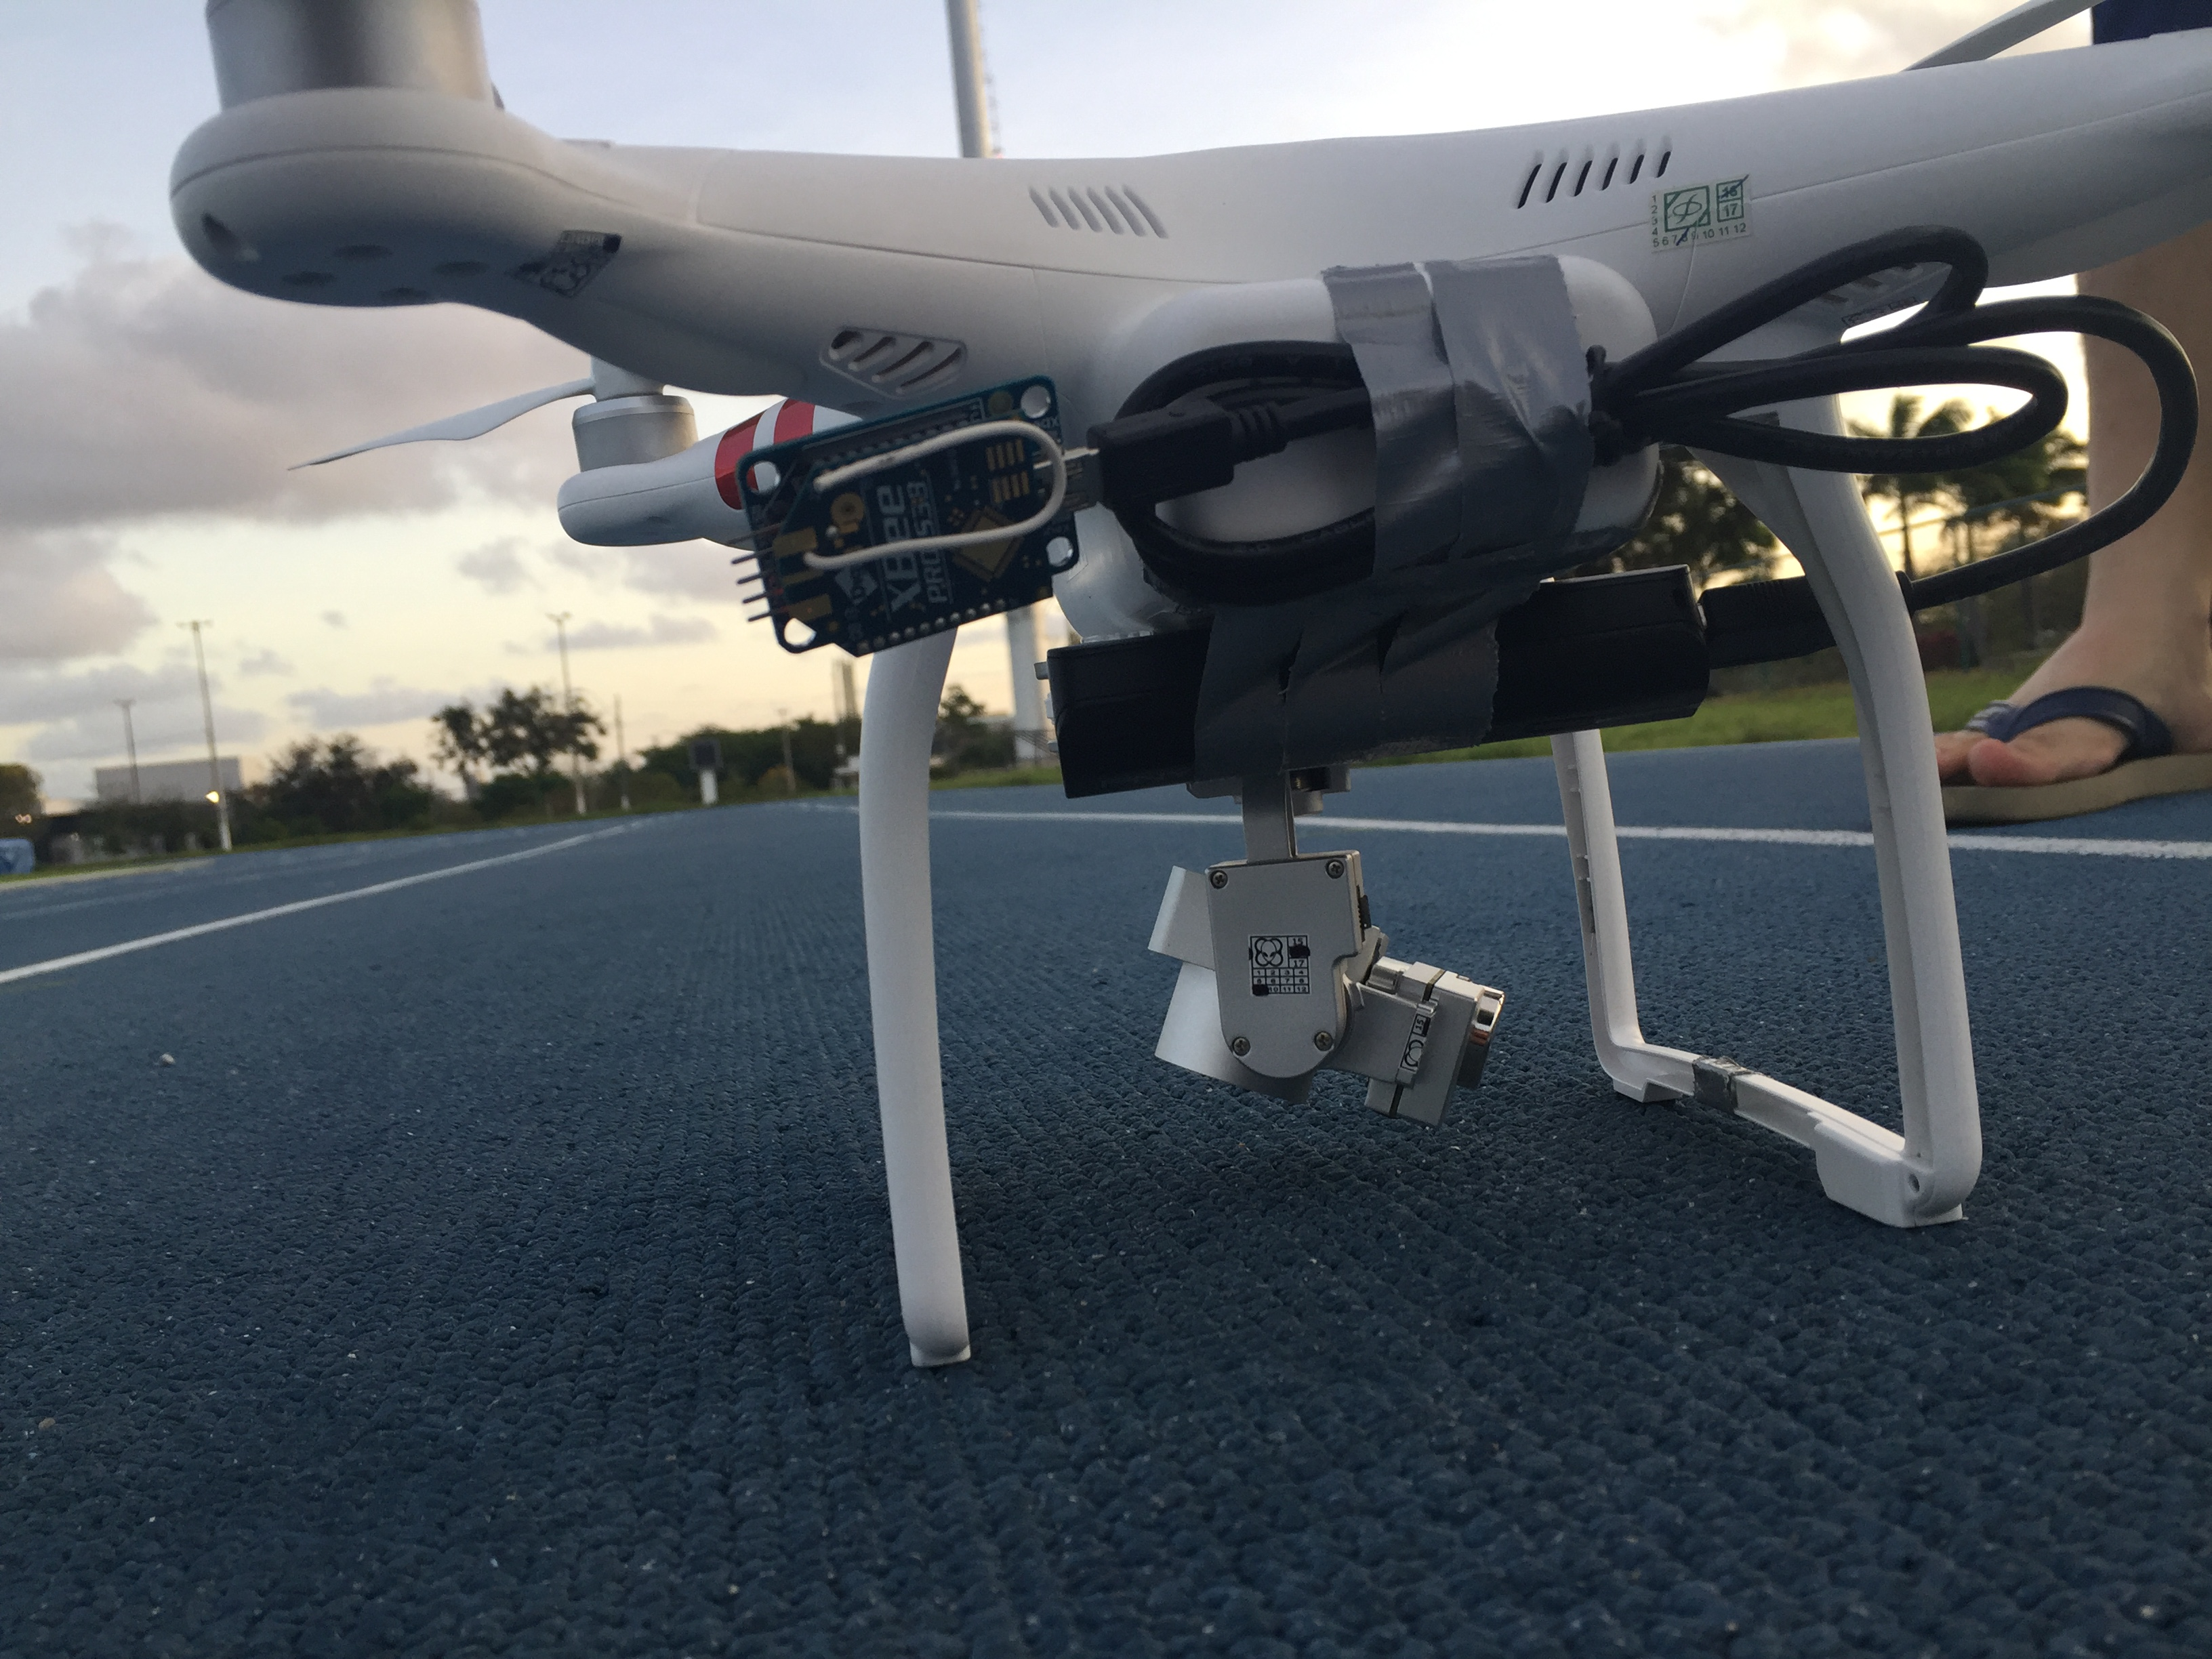
\includegraphics[width=0.7\textwidth]{conjExp.jpg}
\caption{\emph{Phantom 3 Standard} preparado para experimentos.} 
\label{fig:conjExp}
\end{figure}